\documentclass[10pt]{extarticle}
\usepackage[protrusion=true]{microtype}
\usepackage[sfdefault]{FiraSans}
\usepackage[T1]{fontenc}
\usepackage[utf8]{inputenc}
\usepackage{adjustbox}
\usepackage{algorithm}
\usepackage{algorithmic}
\usepackage{amsfonts}
\usepackage{amsmath}
\usepackage{amssymb}
\usepackage[style=apa]{biblatex}
\addbibresource{references.bib}
\usepackage{booktabs}
\usepackage{breqn}
\usepackage{enumitem}
\usepackage{float}
\usepackage{geometry}
\usepackage{graphicx}
\usepackage{hyperref}
\usepackage{lipsum}
\usepackage{longtable}
\usepackage{multirow}
\usepackage{pdfpages}
\usepackage{pgfgantt}
\usepackage{setspace}
\usepackage{subcaption}
\usepackage{tabularx}
\usepackage{tikz}
\usepackage{xcolor}

\DeclareLanguageMapping{english}{english-apa}

\geometry{letterpaper, left=1in, right=1in, top=1in, bottom=1in,}

\definecolor{primary}{RGB}{0,120,215}
\definecolor{secondary}{RGB}{255,87,34}
\definecolor{background}{RGB}{245,245,245}
\definecolor{blue}{RGB}{0,62,126}

\pagecolor{background}

\hypersetup{colorlinks=true, linkcolor=primary, filecolor=secondary, urlcolor=primary, citecolor=black}

\AtBeginBibliography{\hypersetup{urlcolor=black}}

\setstretch{1.15}

\setlength{\bibhang}{0.5in}
\setlength\bibitemsep{1.5\itemsep}

\setlength{\parindent}{0pt}
\setlength{\parskip}{1em}

\nocite{*}

\begin{document}

\newcommand{\mytitlepage}[2]{
    \thispagestyle{empty}

    \begin{tikzpicture}[remember picture, overlay]
        \node [inner sep=0pt] at (current page.center) {#1}; { \node [ anchor=center, inner sep=1.25cm, rectangle, fill=blue!70!white, fill opacity=0, text opacity=1, minimum height=0.2\paperheight, minimum width=\paperwidth, text width=0.8\paperwidth, font=\fontfamily{pnc}\selectfont ] at (current page.center) {#2}; } \node [anchor=south east, outer sep=3pt] at (current page.south east) {\includegraphics[width=0.33\paperwidth]{images/logo.png}};
    \end{tikzpicture}

    \newpage
}

{ \mytitlepage{\includegraphics[width=\paperwidth]{images/background.png}}
    {
        \centering
        \fontfamily{phv}
        \vspace{-200pt} % move title up
        { \Huge
            \bfseries

            Object Detection in Live YouTube Streams

            \par
        }
        \vspace{8pt}
        { \Large
            \bfseries

            Report

            \par
        }
        \vspace{24pt}
        {
            \begin{center}
                \begin{tabular*} {\textwidth}{@{\extracolsep{\fill}}c c c}
                    {\LARGE William Acuna} & {\LARGE Jonathan Agustin} & {\LARGE Alec Anderson}
                \end{tabular*}
            \end{center}
        }
    }
}

\pagenumbering{arabic}

\section{Problem Definition}

The problem we address in this project is the detection and classification of objects in live streaming video content from YouTube. With the growing popularity of live streaming, there's a significant need to analyze these streams effectively. Our focus is on processing these streams to detect various objects they contain. This capability is crucial for applications such as monitoring public spaces for safety, managing traffic flow, and moderating online content.

The necessity of solving this problem arises from the challenges posed by the vast and growing volume of live streaming content. Manual monitoring of these streams is impractical due to their sheer number and the real-time nature of the content. Automated object detection in these streams can provide valuable insights for decision-making in public safety, urban planning, and digital content management.

A computer vision algorithm, specifically the You Only Look Once (YOLO) algorithm, will address the core aspect of this problem: accurately identifying and classifying objects within the video frames of these live streams. The application of YOLO will enable us to process the video data efficiently, identify relevant objects, and categorize them, making the streams more actionable and informative. This project aims to demonstrate how computer vision can transform the way we interact with and manage live video data, making it a subject of both technical interest and practical significance.

\section{Dataset}

Our model used the COCO dataset, which is known for its broad application in object detection, segmentation, and captioning. This dataset is widely used in computer vision research due to its extensive collection of images and annotations across various object categories. COCO is structured into three subsets: Train2017 with 118K images, Val2017 with 5K images, and Test2017 with 20K images. These subsets are important for training, validating, and testing models, respectively.

The COCO dataset includes 80 object categories, ranging from everyday items to more specific objects. Each image in the dataset comes with annotations like bounding boxes and segmentation masks. For our project, we primarily used the Train2017 and Val2017 subsets to train and validate the YOLOv8 model. The COCO dataset's diverse range of annotated images was essential for developing an accurate and efficient object detection model. We managed dataset configurations through a YAML file, outlining essential details like dataset paths and class information, helping with efficient training and validation processes.

\section{Exploratory Data Analysis (EDA)}

We analyzed the COCO dataset to understand its structure. This dataset contains over 330,000 images and 1.5 million object instances. It includes 80 object categories and 91 stuff categories. We examined the distribution of these categories and the annotations for each image. This analysis aimed to identify the variety in the dataset and its implications for our object detection and segmentation goals.

\section{Preprocessing}

The preprocessing primarily involved resizing pictures to 640x640 images. Most of the preprocessing was already done through the dataset maintainers. To confirm, we ran terminal commands on the COCO dataset and searched for corrupted data. We created a \texttt{ModelManager} class for managing the dataset during model training. The class sets up TensorBoard for logging, managed model directories, and oversaw the training process. This overall approach transformed the dataset to be used effectively in our project.

\section{Modeling Methods}

Our object detection system was built around the YOLOv8 algorithm, the latest iteration in the YOLO series known for its object detection capabilities. YOLOv8's architecture, a convolutional neural network, is split into two primary parts: the backbone and the head. The backbone is based on a modified CSPDarknet53 architecture, featuring 53 convolutional layers enhanced with cross-stage partial connections for improved information flow. This structure supports the intricate processing required for correct object detection. The head of YOLOv8 comprises multiple convolutional layers followed by connected layers. These are pivotal in predicting bounding boxes, objectness scores, and class probabilities. A significant feature of YOLOv8's head is the integration of a self-attention mechanism. This addition lets the model selectively focus on different parts of an image, adjusting the importance of features based on their relevance to the detection task.

YOLOv8 excels in multi-scaled object detection. It uses a feature pyramid network to detect objects at various scales within an image. This capability is essential for accurately identifying both large and small objects, making YOLOv8 versatile for diverse object detection scenarios. YOLOv8's architecture supports multiple backbones like EfficientNet, ResNet, and CSPDarknet, offering flexibility in model selection based on specific needs. The customizability of YOLOv8's architecture is another strength, enabling changes to the model's structure and parameters to tailor it for various applications ranging from autonomous vehicles and surveillance to retail and medical imaging.

\subsection{Training}

The training code includes a \texttt{ModelManager} class, which encapsulates the functionality needed to manage the model's lifecycle, including downloading configuration files, setting up TensorBoard for logging, and training the model.

The \texttt{train\_model} method within the \texttt{ModelManager} class is responsible for initiating the training process. It checks if a pre-trained model exists and, based on the \texttt{resume} flag, either resumes training or starts afresh using the specified model configuration. The training uses the COCO dataset, as indicated by the \texttt{data} argument pointing to ``coco.yaml''. The model is trained for a small number of epochs (3) with a batch size of 1 and an image size of 640 pixels. The \texttt{save\_period} argument ensures that the model is saved after every epoch. If a CUDA-capable GPU is available, the model utilizes it to accelerate the training process.

Several important arguments in the script control various aspects of the training:

\begin{itemize}
    \item \texttt{epochs}: The number of complete passes through the dataset.
    \item \texttt{batch}: The number of samples processed before the model is updated.
    \item \texttt{imgsz}: The size of the images that the model will process.
    \item \texttt{optimizer}: The optimization algorithm used for training.
    \item \texttt{device}: The device on which the model will be trained, e.g., a CUDA-enabled GPU.
    \item \texttt{project} and \texttt{name}: The directory and name for saving the trained model.
    \item \texttt{resume}: A flag indicating whether to resume training from the last checkpoint.
    \item \texttt{amp}: Automatic Mixed Precision for faster training on compatible hardware.
    \item \texttt{iou}: The Intersection Over Union threshold used for evaluating object detection performance.
    \item \texttt{max\_det}: The maximum number of detections allowed per image.
    \item \texttt{plots}: Whether to generate plots during training, such as precision-recall curves.
\end{itemize}

\section{Validation}

In validating our model with Ultralytics YOLOv8's Val mode, we used metrics such as Precision, Recall, mAP50, and mAP50-95. This approach allowed us to assess the model's object detection accuracy and speed across different classes in the COCO dataset. The Val mode's automatic retention of training settings simplified the process, ensuring consistent testing conditions.

The validation provided class-wise performance data, visual charts like F1 Score and Precision-Recall Curves, and confusion matrices. These outputs helped us understand the model's strengths and weaknesses, guiding adjustments in hyperparameters. We stored all results for ongoing analysis and model refinement.
\section{Performance Metrics Analysis}

We evaluated the accuracy and efficiency of our object detection model using several metrics. These metrics provide insights into the model's ability to identify and localize objects and its handling of false positives and negatives.

\subsection{Key Metrics}

\begin{itemize}
    \item \textbf{Intersection over Union (IoU)}: Measures the overlap between predicted and ground truth bounding boxes, indicating localization accuracy.
    \item \textbf{Average Precision (AP)}: Reflects the model's precision and recall, calculated as the area under the precision-recall curve.
    \item \textbf{Mean Average Precision (mAP)}: Averages the AP values across multiple object classes, important for models detecting various classes.
    \item \textbf{Precision and Recall}: Precision assesses the model's ability to minimize false positives, while recall measures its ability to detect all instances of a class.
    \item \textbf{F1 Score}: Balances precision and recall, important for models where both false positives and negatives are critical.
\end{itemize}

\subsection{Calculating and Interpreting Metrics for YOLOv8}
To compute these metrics, we used YOLOv8's validation mode. This process involves processing a validation dataset and returning various performance metrics.

\subsubsection{Model Validation Outputs}
\begin{itemize}
    \item \textbf{Class-wise Metrics}: Includes precision, recall, and mAP for each class, providing a detailed view of model performance per category.
    \item \textbf{Speed Metrics}: Analyzes the time taken for different stages of validation, crucial in real-time detection scenarios.
    \item \textbf{COCO Metrics}: Additional precision and recall metrics for the COCO dataset, giving insights into performance across different object sizes and IoU thresholds.
    \item \textbf{Visual Outputs}: Includes F1 score curve, precision-recall curve, precision and recall curves, confusion matrices, and validation batch images. These visuals aid in understanding the model's detection and classification accuracy.
\end{itemize}

\subsubsection{Results Interpretation}
\begin{itemize}
    \item \textbf{Low mAP} might suggest a need for model refinement.
    \item \textbf{Low IoU} indicates poor object localization, possibly requiring different bounding box methods.
    \item \textbf{Low Precision} implies excessive false detections, which can be reduced by adjusting confidence thresholds.
    \item \textbf{Low Recall} indicates missed real objects, potentially improvable with better feature extraction or more data.
    \item \textbf{Class-specific AP scores} can highlight specific classes where the model underperforms.
\end{itemize}

\section{Model Results}

During tests, our model identified objects in several settings. It picked out everyday items like trains and handbags, along with animals such as elephants and zebras, in an urban scene. The model worked well with objects that stood out in shape and color. In a beach scene, the model distinguished between still objects and those in motion like airplanes and trains. It also spotted smaller items, like kites. This shows the model's range in detecting objects of different sizes. Lastly, the model handled a mix of moving and stationary objects. It detected them with a reasonable degree of accuracy, proving it can work in various conditions. The tests showed the model's ability to detect objects consistently.

\begin{figure}[H]
    \centering
    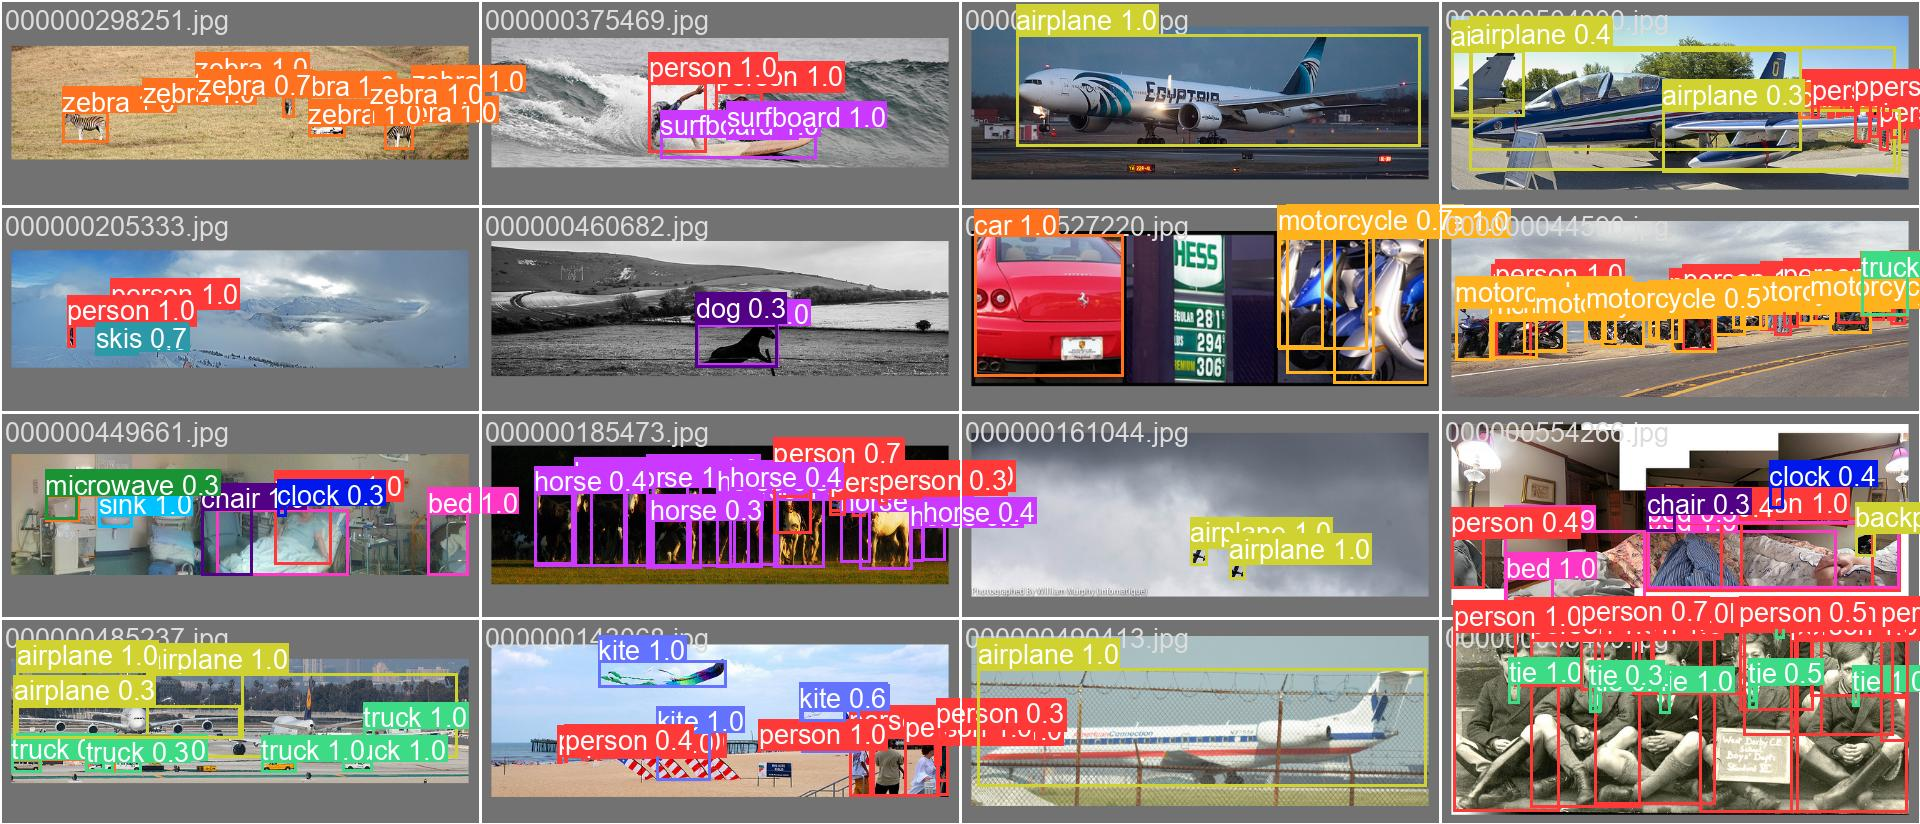
\includegraphics[width=0.6\textwidth]{images/val_batch0_pred.jpg}
    \\
    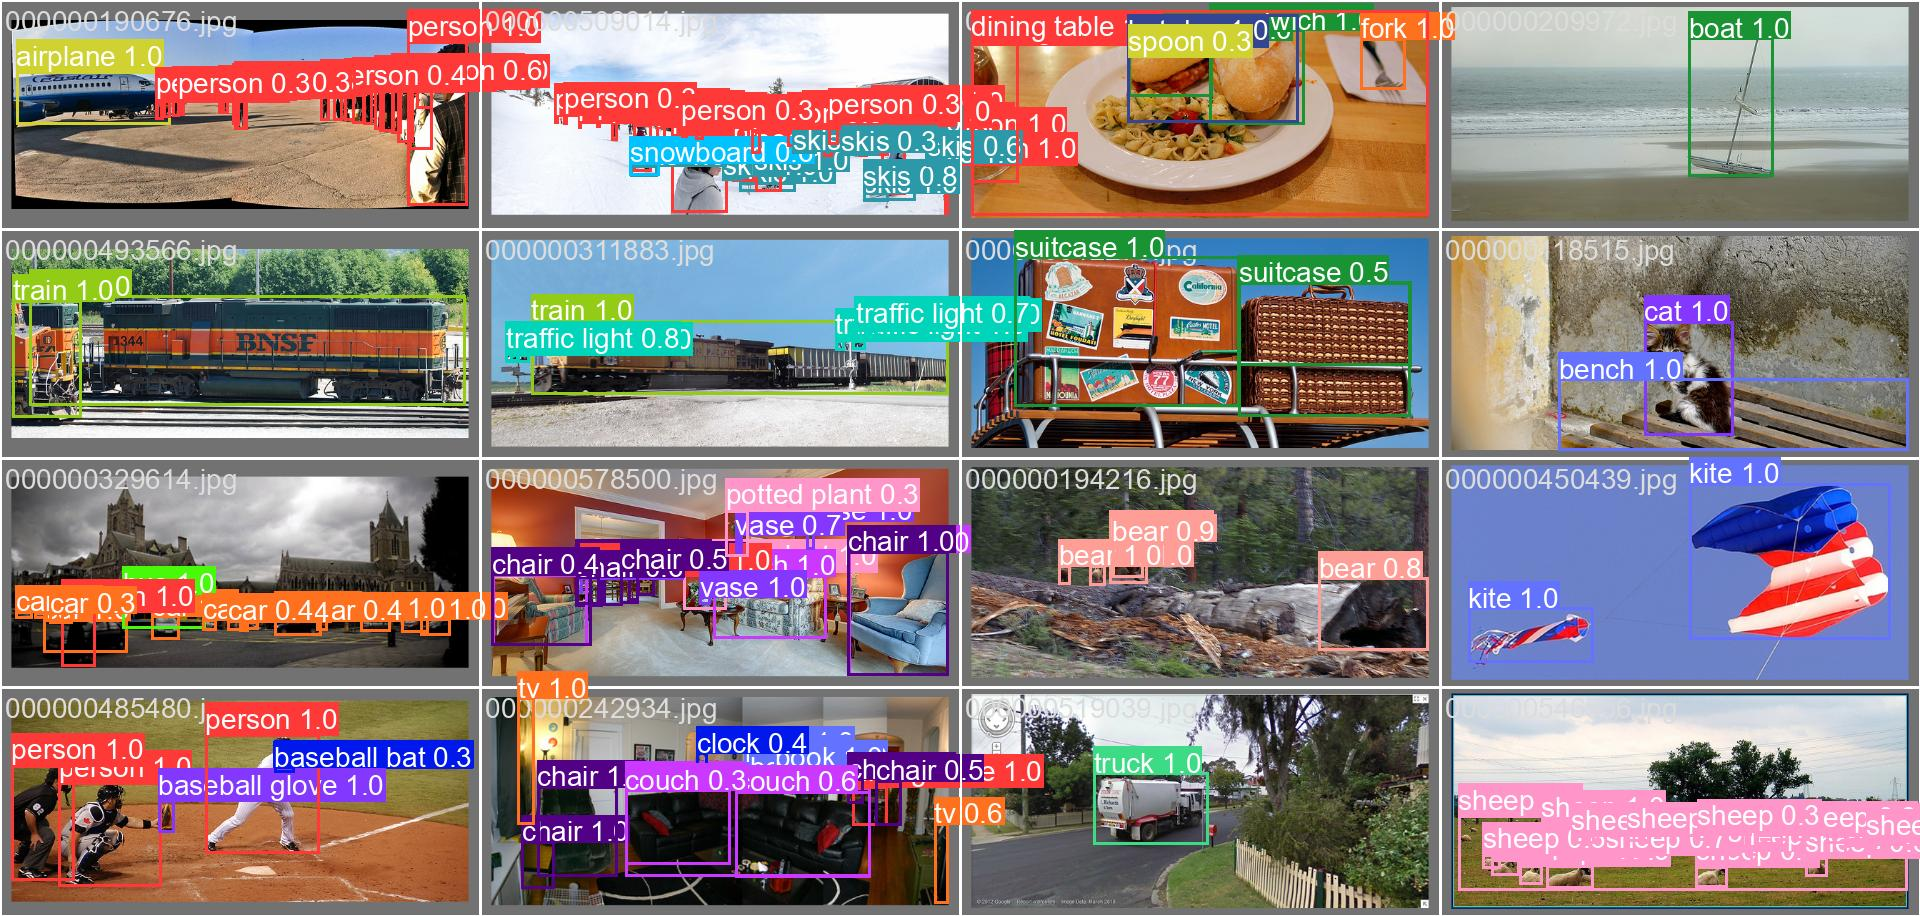
\includegraphics[width=0.6\textwidth]{images/val_batch1_pred.jpg}
    \\
    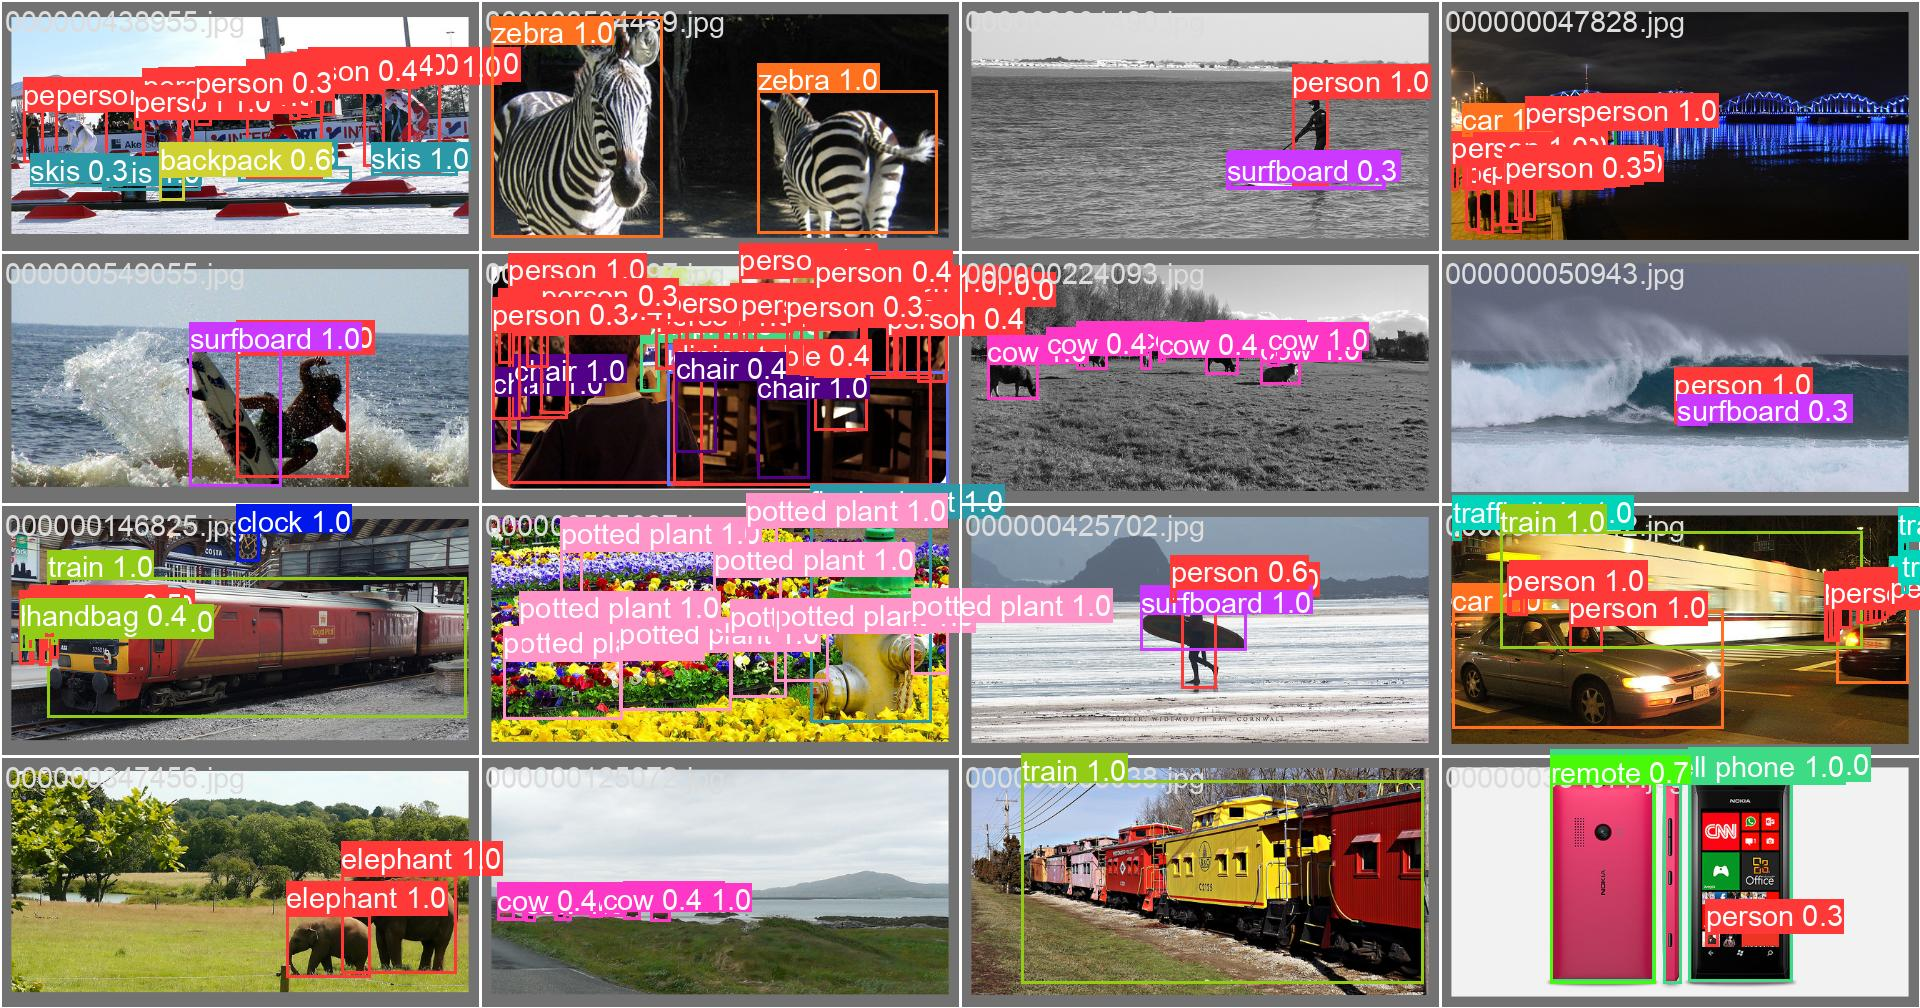
\includegraphics[width=0.6\textwidth]{images/val_batch2_pred.jpg}
    \label{fig:combined_environments}
\end{figure}


\subsection{Graphs}


\begin{figure}[H]
    \centering
    \includegraphics[width=0.8\textwidth]{images/results.png}
    \end{figure}

The provided results from our model training over three epochs presents an encouraging trend of performance enhancement across various parameters. The 'Box Loss' graphs for both training and validation indicate a steady decline, which signifies an improvement in the model's ability to predict the correct bounding boxes around objects. A lower box loss correlates to a higher accuracy in locating the objects within the images.

Similarly, the 'Class Loss' for training and validation shows a downward slope, reflecting the model's growing competence in correctly classifying the objects. Lower classification loss means the model is getting better at identifying what the objects are. 'DFL Loss' or Detection Family Loss, which encapsulates several aspects of detection quality, also displays a consistent decrease. This suggests that the model's understanding of object features and their interrelations is maturing, leading to better detection results.

In terms of 'Precision', there is a noticeable upward trend across epochs. Higher precision points to a higher ratio of true positive detections versus false positives, which is crucial for the practical application of the model, ensuring that it is reliable when deployed in real-world scenarios. 'Recall' also exhibits an increasing trend, which is indicative of the model's ability to detect all relevant instances of objects. An increase in recall means that the model is less likely to miss objects that should be detected.

Lastly, the 'mAP' (mean Average Precision) scores, both for mAP50 and mAP50-95, are on the rise. These metrics are particularly important because they provide a single-figure measure of the quality of object detections made by the model, not just in terms of their presence, but also their location and classification across a range of sizes and difficulties. The mAP50 metric shows the model's precision over a 50\% threshold for Intersection over Union (IoU), while mAP50-95 averages mAP calculated at different IoU thresholds, from 50\% to 95\%. The growth in these values suggests that the model is not only improving in recognizing objects but is also doing so with a greater agreement to the ground truth data, which is promising for its application in environments where precision is critical.

During the evaluation of our model, we relied on various performance curves to understand its predictive capabilities and to identify areas for improvement. Below we discuss the significance of the Precision-Recall, Precision-Confidence, F1-Confidence, and Recall-Confidence curves generated during our testing phase. These curves collectively provide a comprehensive view of the model's strengths and weaknesses in terms of its prediction capabilities. They are instrumental in fine-tuning the model to achieve the best performance possible on unseen data.

\section{Findings}

\subsection{Deployed Examples}

\textbf{Example 1: California Beach at Sunset}
We tested our model on a live stream from a California beach at sunset. The model effectively identified bicycles and people, demonstrating good performance even in challenging lighting. Accurate bounding boxes were generated, with a color-coded key for clarity. However, it misclassified two lifeguard towers as boats, indicating a need for improvement in object differentiation.

\begin{figure}[H]
\centering
\includegraphics[width=0.8\textwidth]{images/pic1.png}
\caption{Object detection on a California beach at sunset.}
\end{figure}

\textbf{Example 2: Overcast Conditions in Brazil}
In Brazil, under overcast conditions, the model showed proficiency in classifying chairs and umbrellas, even with overlapping objects. It detected almost every person present, missing only one individual in the background. This test underscores the model's capability in handling complex scenes with multiple objects.

\begin{figure}[H]
\centering
\includegraphics[width=0.8\textwidth]{images/pic2.png}
\caption{Object detection on an overcast beach in Brazil.}
\end{figure}

\textbf{Example 3: Crowded Bar Scene}
The crowded bar scene test was critical for assessing the model in dense areas. The model successfully identified people and objects like handbags and bottles. However, it faced challenges with overlapping bounding boxes and false positives, highlighting areas for refinement in crowded environments.

\begin{figure}[H]
\centering
\includegraphics[width=0.8\textwidth]{images/pic3.png}
\caption{Object detection in a crowded bar scene.}
\end{figure}

\subsection{Challenges and Insights}
During development, we shifted from Streamlit to Gradio for a more interactive interface. The tests, particularly in the crowded bar scene, revealed precision issues. Despite these challenges, the model's resilience to varying lighting conditions was a positive outcome. Inaccuracies in object localization in dense scenes indicate the need for improved distinction between closely situated objects.

\subsection{Potential Applications}
The system shows promise for surveillance security and traffic management. In security, it can detect threats or unauthorized activities, such as unattended luggage in airports. For urban planning, it can analyze traffic patterns and pedestrian flows, aiding in smarter traffic control system designs. Additionally, the project is beneficial for creating labeled datasets for diverse environments, contributing to the research community.

\subsection{Future Improvements}
Future enhancements will focus on increasing accuracy and real-time processing. This involves refining bounding box precision, enhancing object classification, and reducing false positives in dense environments. Improving real-time processing is crucial for timely decision-making and responsiveness in deployment.

\section{Conclusion}
Our tests across different scenarios demonstrated the adaptability and practicality of our object detection system, particularly with the 'yolov8x' model. The system's ability to handle diverse lighting conditions was a significant achievement. Future improvements will concentrate on object localization and classification accuracy in crowded scenes and enhancing real-time processing efficiency. These enhancements are pivotal for advancing the system's utility across various sectors.

\newpage

\printbibliography

\newpage


\section{Appendix}

\subsection{Project Artifacts}

\begin{itemize}

    \item Deployed Model Application:
    \begin{itemize}
        \item \url{https://huggingface.co/spaces/aai521-group6/youtube-object-detection}
    \end{itemize}

    \item Hugging Face Model
    \begin{itemize}
        \item \url{https://huggingface.co/aai521-group6/yolov8x-coco}
    \end{itemize}

    \item GitHub Repository
    \begin{itemize}
        \item \url{https://github.com/aai521-group6/project}
    \end{itemize}
\end{itemize}

\subsection{Project Code}

\newpage

\clearpage
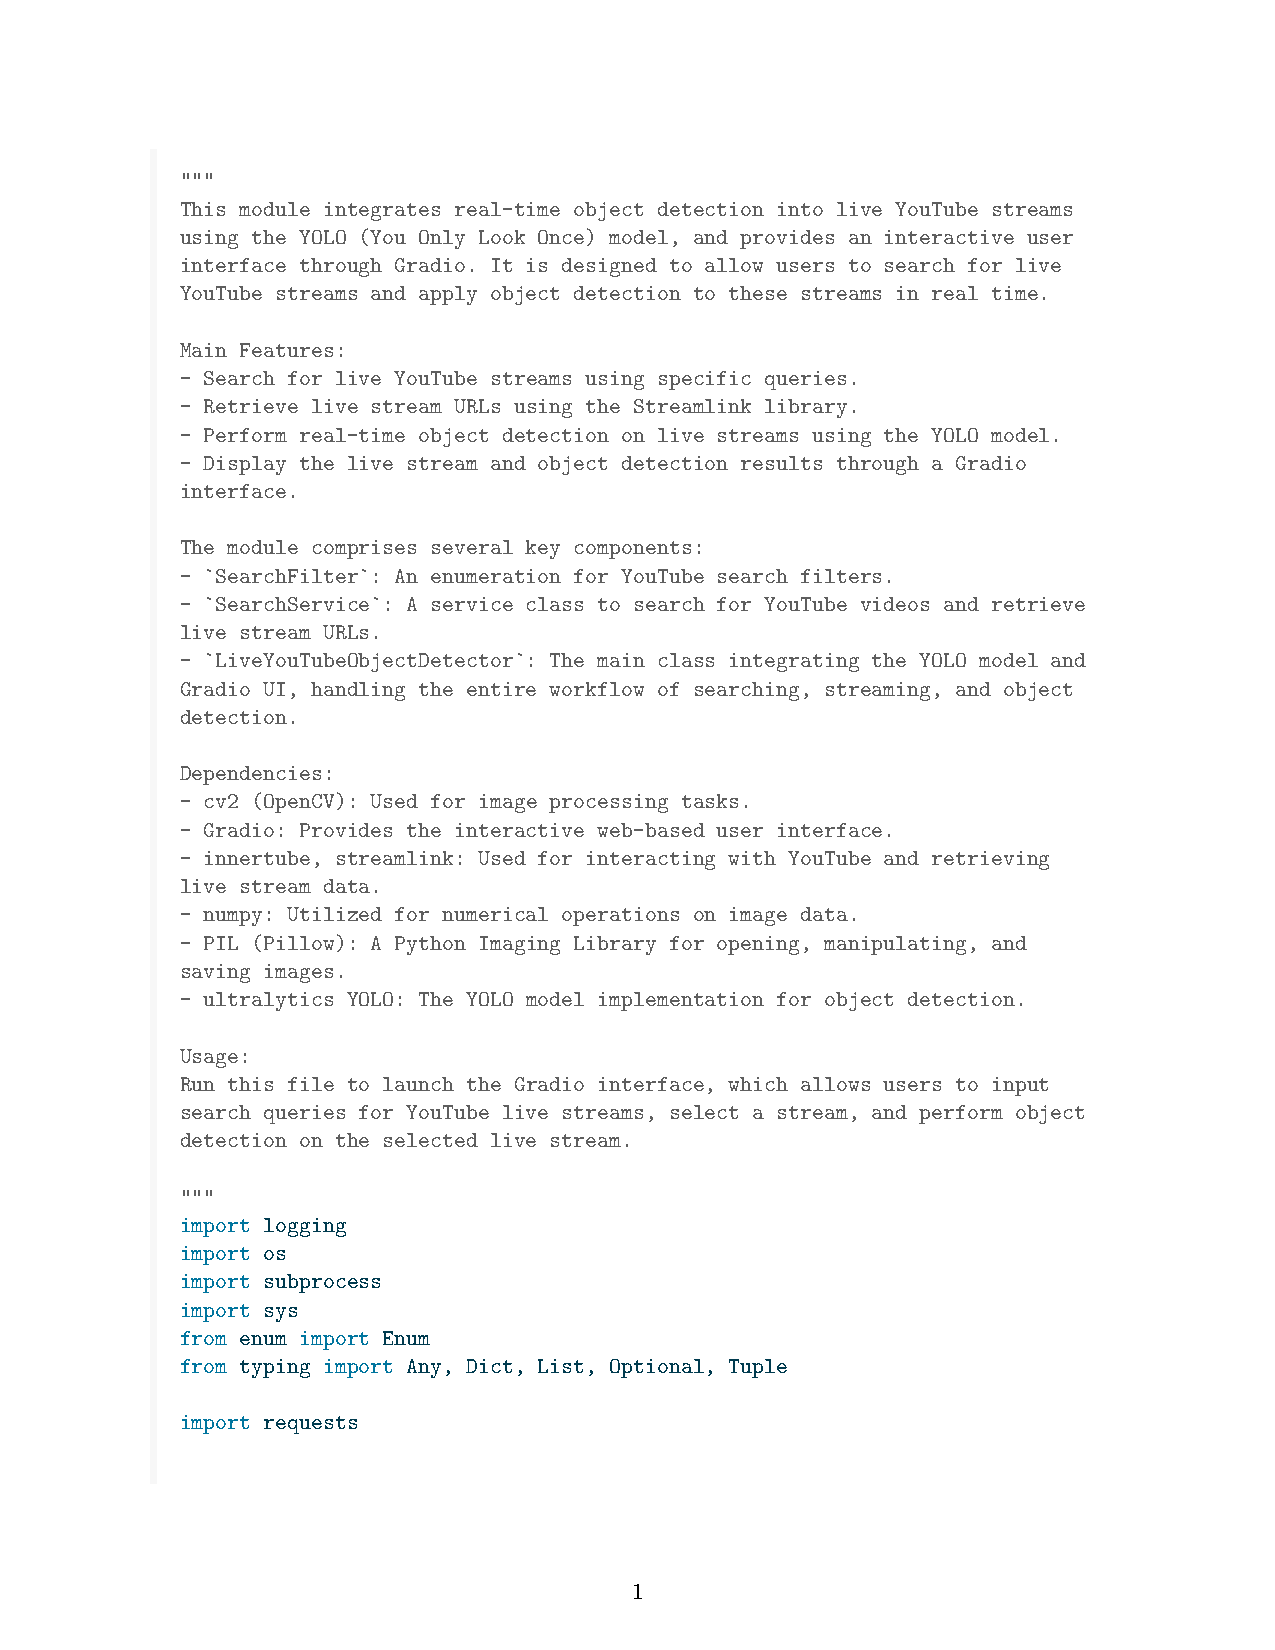
\includepdf[pages=-, fitpaper=true]{code.pdf}

\end{document}
